\documentclass[border=6pt]{standalone}
\usepackage{amsmath}
\usepackage{tikz}
\usepackage{pgfplots}
\pgfplotsset{compat=1.18}
\usetikzlibrary{arrows.meta,calc,positioning}
\begin{document}
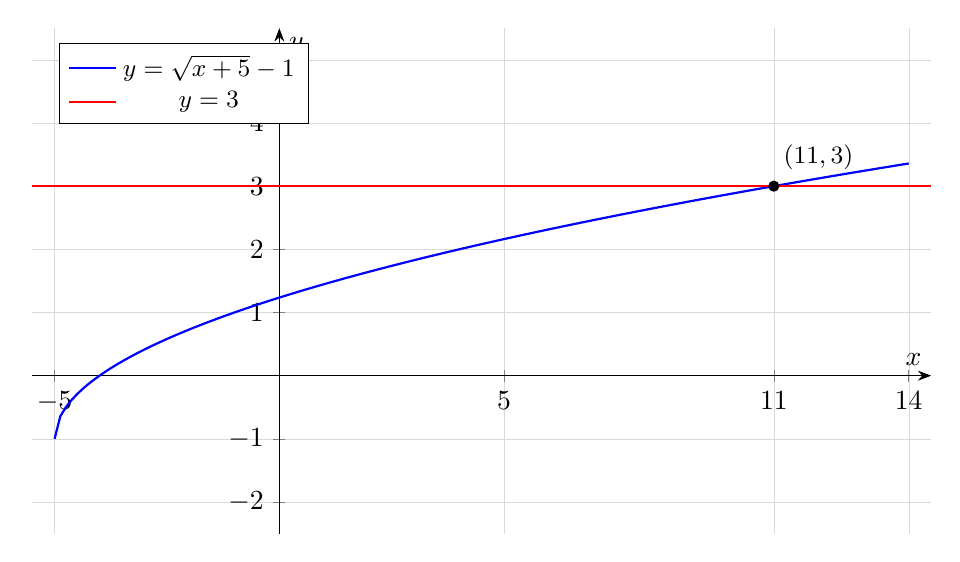
\begin{tikzpicture}
\begin{axis}[
    axis lines = middle,
    xlabel = {$x$}, ylabel = {$y$},
    xmin=-5.5, xmax=14.5, ymin=-2.5, ymax=5.5,
    xtick={-5,0,5,11,14},
    ytick={-2,-1,0,1,2,3,4,5},
    grid=both,
    grid style={line width=.1pt, draw=gray!30},
    width=13cm, height=8cm,
    axis line style={-Stealth},
    legend pos=north west,
    legend style={font=\small},
]
% y = sqrt(x+5) - 1, domain x >= -5
\addplot[domain=-5:14, samples=150, thick, blue] {sqrt(x+5)-1};
\addlegendentry{$y=\sqrt{x+5}-1$}

% horizontal line y = 3
\addplot[domain=-5.5:14.5, samples=2, thick, red] {3};
\addlegendentry{$y=3$}

% intersection point (11,3)
\addplot[only marks, mark=*, mark size=1.8pt, black] coordinates {(11,3)};
\node[anchor=south west] at (axis cs:11,3.1) {\small $(11,3)$};

\end{axis}
\end{tikzpicture}
\end{document}
